% Converted from Microsoft Word to LaTeX
% by Chikrii Softlab Word2TeX converter (version 3.0)
% Copyright (C) 1999-2003 Chikrii Softlab. All rights reserved.
% http://www.chikrii.com
% mailto: info@chikrii.com
% License: infern0 /

\documentclass{article}
\usepackage{latexsym}
\usepackage{graphicx}

\begin{document}

\begin{center}
\textbf{OpenCV Reference Manual}
\end{center}

\begin{center}
v2.4
\end{center}

\begin{center}
June, 2012
\end{center}

\newpage

\begin{table}[htbp]
\begin{center}
\begin{tabular}{|p{426pt}|}
\hline
 \\
\hline
\end{tabular}
\label{tab1}
\end{center}
\end{table}


\section { General Information }
The OpenCV OCL module is a set of classes and functions to utilize OpenCL compatible device. In theroy, it supports any OpenCL 1.1 compatible device, but we only test it on AMD's and NVIDIA's GPU at this stage. The OpenCV OCL module includes utility functions, low-level vision primitives, and high-level algorithms. The utility functions and low-level primitives provide a powerful infrastructure for developing fast vision algorithms taking advangtage of OCL whereas the high-level functionality includes some state-of-the-art algorithms(such as stereo correspondence, face detector) ready to be used by the application developers.

The OpenCV OCL module is designed as a host-level API plus device-level kernels. The device-level kernels are collected as strings at OpenCV compile time and are compiled at runtime, so it need OpenCL runtime support. To correctly run the OpenCV OCL module, make sure you have OpenCL runtime provided by your device vendor, which is device driver normally.

The OpenCV OCL module is designed for ease of use and does not require any knowledge of OpenCL. Though, such a knowledge will certainly be useful to handle non-trivial cases or achieve the highest performance. It is helpful to understand the cost of various operations, what the OCL does, what the preferred data formats are, and so on. Since there is data transfer between OpenCL host and OpenCL device, the recommanded operation is transfer data from host -> ocl::func1 -> ocl::func2 -> .... -> ocl::funcN -> transfer data to host if needed, not transfer data from host -> ocl::func1 -> transfer data to host -> transfer data from host -> ocl::func2 .....

To enable OCL support, configure OpenCV using CMake with WIHT\_OPENCL=ON. When the flag is set and if OpenCL SDK is installed, the full-featured OpenCV OCL module is built. Otherwis, the module may be not built.

Right now, the user should define the cv::ocl::Info class in the application and call cv::ocl::getDevice before any cv::ocl::func. This operation initialize OpenCL runtime and set the first found device as computing device. If there are more than one device and you want to use undefault device, you can call cv::ocl::setDevice then.

In the current version, all the thread share the same context and device so the multi-devices are not supported. We will add this feature soon.

\section{utility functions}

\subsection{Info}
class CV\_EXPORTS Info

\{

public:

	struct Impl;

	Impl *impl;

	Info();

	Info(const Info \&m);

	~Info();

	void release();

	Info \&operator = (const Info \&m);

\};

this class sould be maintained by the user and be passed to getDevice

\subsection{int getDevice}


parameters: 

std::vector<Info>\& oclinfo  it must not be NULL

int devicetype = CVCL\_DEVICE\_TYPE\_GPU The device type you want to use, the default value is GPU, other alternatives are CVCL\_DEVICE\_TYPE\_DEFAULT, CVCL\_DEVICE\_TYPE\_CPU, CVCL\_DEVICE\_TYPE\_ACCELERATOR, CVCL\_DEVICE\_TYPE\_ALL

return value: the number of devices found, must be greater than 0.

the function must be called before any other cv::ocl::functions, it initialize ocl runtime

\subsection{void setDevice}


parameters:

Info \&oclinfo  the selected OpenCL platform

int devnum = 0 the selected OpenCL device under this platform

\subsection{void setBinpath}


parameters:

const char *path the path of OpenCL kernel binaries

If you call this function and set a valid path, the OCL module will save the compiled kernel to the address in the first time and reload the binary since that. It can save compilation time at the runtime.


\section{1 core. The Core Functionality}
\label{sec:mylabel1}
\subsection{1.1 Basic Structures}
\label{subsec:mylabel1}
\subsubsection{cv::ocl::convertTo}
\label{subsubsec:mylabel1}
Converts array to another datatype with optional scaling.

Supports CV{\_}8UC1,CV{\_}8UC4,CV{\_}32SC1,CV{\_}32SC4,CV{\_}32FC1,CV{\_}32FC4.

\textbf{m }The destination matrix. If it does not have a proper size or type
before the operation, it will be reallocated

\textbf{rtype }The desired destination matrix type, or rather, the depth
(since the number of channels will be the same with the source one). If
rtype is negative, the destination matrix will have the same type as the
source.

\textbf{alpha }The optional scale factor

\textbf{beta }The optional delta, added to the scaled values.

The method converts source pixel values to the target datatype. saturate
cast$<>$ is applied in the end to avoid possible overflows:
\[
m(x,y)=saturate\_cast<rType>(\alpha (\ast this)(x,y)+\beta )
\]
\newpage

\subsubsection{cv::ocl::copyTo}
\label{subsubsec:mylabel2}
Copies the matrix to another one.

Supports CV{\_}8UC1,CV{\_}8UC4,CV{\_}32SC1,CV{\_}32SC4,CV{\_}32FC1,CV{\_}32FC4.

\textbf{m }The destination matrix. If it does not have a proper size or type
before the operation, it will bereallocated

\textbf{mask }The operation mask. Its non-zero elements indicate, which
matrix elements need to be copied

The method copies the matrix data to another matrix. Before copying the
data, the method invokes

so that the destination matrix is reallocated if needed. While m.copyTo(m);
will work as expected, i.e. will have no effect, the function does not
handle the case of a partial overlap between the source and the destination
matrices.

When the operation mask is specified, and the Mat::create call shown above
reallocated the matrix, the newly allocated matrix is initialized with all
0's before copying the data.

\newpage

\subsubsection{cv::ocl::setTo}
\label{subsubsec:mylabel3}
Sets all or some of the array elements to the specified value.

Supports CV{\_}8UC1,CV{\_}8UC4,CV{\_}32SC1,CV{\_}32SC4,CV{\_}32FC1,CV{\_}32FC4.

\textbf{s }Assigned scalar, which is converted to the actual array type

\textbf{mask }The operation mask of the same size as *this

This is the advanced variant of Mat::operator=(const Scalar{\&} s) operator.

\newpage

\subsection{1.2 operations on Arrays}
\label{subsec:mylabel2}
\subsubsection{cv::ocl::absdiff}
\label{subsubsec:mylabel4}
Computes per-element absolute difference between two arrays or between array
and a scalar.

Supports all data types except CV{\_}8SC1, CV{\_}8SC2, CV8SC3 and
CV{\_}8SC4.

\textbf{src1 }The first input array

\textbf{src2 }The second input array, must be the same size and same type as
src1

\textbf{sc }Scalar, the second input parameter

\textbf{dst }The destination array, it will have the same size and same type
as src1

The functions absdiff compute:

\begin{itemize}
\item absolute difference between two arrays
\end{itemize}
dst(I) = saturate($\vert $src1(I) - src2(I)$\vert )$

\begin{itemize}
\item or absolute difference between array and a scalar:
\end{itemize}
dst(I) = saturate($\vert $src1(I) -- sc$\vert )$

Where I is multi-dimensional index of array elements. In the case of
multi-channel arrays each channel is processed independently.

\newpage

\subsubsection{cv::ocl::add}
\label{subsubsec:mylabel5}
Computes the per-element sum of two array and a scalar.

Supports all data types except CV{\_}8SC1, CV{\_}8SC2, CV8SC3 and
CV{\_}8SC4.

\textbf{src1} The first source array

\textbf{src2} The second source array. It must have the same size and same
type as src1

\textbf{sc} Scalar; the second input parameter

\textbf{dst } The destination array; it will have the same size and same
type as src1

\textbf{mask} The optional operation mask, 8-bit single channel array;
specifies elements of the destination array to be changed

The functions add compute:

\begin{itemize}
\item the sum of two arrays:
\end{itemize}
dst(I) = saturate(src1(I) + src2(I)) if mask(I) 6= 0

\begin{itemize}
\item or the sum of array and a scalar:
\end{itemize}
dst(I) = saturate(src1(I) + sc) if mask(I) 6= 0

where I is multi-dimensional index of array elements.

The first function in the above list can be replaced with matrix
expressions:

in the case of multi-channel arrays each channel is processed independently.

\newpage

\subsubsection{cv::ocl::bitwise{\_}and }
\label{subsubsec:mylabel6}
Calculates per-element bit-wise conjunction of two arrays and an array and a
scalar.

Supports all data types except CV{\_}64FC1, CV{\_}64FC2, CV64FC3 and
CV{\_}64FC4.

\textbf{src1 }The first source array

\textbf{src2 }The second source array. It must have the same size and same
type as src1

\textbf{sc }Scalar; the second input parameter

\textbf{dst }The destination array; it will have the same size and same type
as src1

\textbf{mask }The optional operation mask, 8-bit single channel array;
specifies elements of the destination array to be changed

The functions bitwise and compute per-element bit-wise logical conjunction:

\begin{itemize}
\item of two arrays:
\end{itemize}
\[
\mbox{dst}\left( I \right)=\mbox{src1}\left( I \right)\wedge
\mbox{src2}\left( I \right)\mbox{ if mask}\left( I \right)\ne 0
\]
\begin{itemize}
\item or array and a scalar:
\end{itemize}
\[
\mbox{dst}\left( I \right)=\mbox{src1}\left( I \right)\wedge \mbox{sc if
mask}\left( I \right)\ne 0
\]
In the case of floating-point arrays their machine-specific bit
representations (usually IEEE754-compliant) are used for the operation, and
in the case of multi-channel arrays each channel is processed independently.

\newpage

\subsubsection{cv::ocl::bitwise{\_}not }
\label{subsubsec:mylabel7}
Inverts every bit of array.

Supports CV{\_}8U, CV{\_}8S, CV{\_}16U, CV{\_}16S, CV{\_}32S, CV{\_}32F data
types.

\textbf{src1 }The source array

\textbf{dst }The destination array; it is reallocated to be of the same size
and the same type as src

\textbf{mask }The optional operation mask, 8-bit single channel array;
specifies elements of the destination array to be changed

The functions bitwise not compute per-element bit-wise inversion of the
source array:
\[
\mbox{dst}\left( I \right)=\neg \mbox{src}\left( I \right)
\]
In the case of floating-point source array its machine-specific bit
representation (usually IEEE754-compliant) is used for the operation. in the
case of multi-channel arrays each channel is processed independently.

\newpage

\subsubsection{cv::ocl::bitwise{\_}or }
\label{subsubsec:mylabel8}
Calculates per-element bit-wise disjunction of two arrays and an array and a
scalar.

Supports all data types except CV{\_}64FC1,CV{\_}64FC2,CV64FC3 and
CV{\_}64FC4.

\textbf{src1 }The first source array

\textbf{src2 }The second source array. It must have the same size and same
type as src1

\textbf{sc }Scalar; the second input parameter

\textbf{dst }The destination array; it is reallocated to be of the same size
and the same type as src1

\textbf{mask }The optional operation mask, 8-bit single channel array;
specifies elements of the destination array to be changed

The functions bitwise or compute per-element bit-wise logical disjunction

\begin{itemize}
\item of two arrays:
\end{itemize}
\[
\mbox{dst}\left( I \right)=\mbox{src1}\left( I \right)\vee \mbox{src2}\left(
I \right)\mbox{ if mask}\left( I \right)\ne 0
\]
\begin{itemize}
\item or array and a scalar:
\end{itemize}
\[
\mbox{dst}\left( I \right)=\mbox{src1}\left( I \right)\vee \mbox{sc if
mask}\left( I \right)\ne 0
\]
In the case of floating-point arrays their machine-specific bit
representations (usually IEEE754-compliant) are used for the operation. in
the case of multi-channel arrays each channel is processed independently.

\newpage

\subsubsection{cv::ocl::bitwise{\_}xor }
\label{subsubsec:mylabel9}
Calculates per-element bit-wise ``exclusive or'' operation on two arrays and
an array and a scalar.

Supports all data types except CV{\_}64FC1,CV{\_}64FC2,CV64FC3 and
CV{\_}64FC4.

\textbf{src1 }The first source array

\textbf{src2 }The second source array. It must have the same size and same
type as src1

\textbf{sc }Scalar; the second input parameter

\textbf{dst }The destination array; it is reallocated to be of the same size
and the same type as src1

\textbf{mask }The optional operation mask, 8-bit single channel array;
specifies elements of the destination array to be changed

The functions bitwise xor compute per-element bit-wise logical ''exclusive
or'' operation

\begin{itemize}
\item on two arrays:
\end{itemize}
\[
\mbox{dst}\left( I \right)=\mbox{src1}\left( I \right)\oplus
\mbox{src2}\left( I \right)\mbox{ if mask}\left( I \right)\ne 0
\]
\begin{itemize}
\item or array and a scalar:
\end{itemize}
\[
\mbox{dst}\left( I \right)=\mbox{src1}\left( I \right)\oplus \mbox{sc if
mask}\left( I \right)\ne 0
\]
In the case of floating-point arrays their machine-specific bit
representations (usually IEEE754-compliant) are used for the operation. in
the case of multi-channel arrays each channel is processed independently.

\newpage

\subsubsection{cv::ocl::cartToPolar }
\label{subsubsec:mylabel10}
Calculates the magnitude and angle of 2d vectors.

Supports only CV{\_}32F, CV{\_}64F data types.

\textbf{x }The array of x-coordinates; must be single-precision or
double-precision floating-point array

\textbf{y }The array of y-coordinates; it must have the same size and same
type as x

\textbf{magnitude }The destination array of magnitudes of the same size and
same type as x

\textbf{angle }The destination array of angles of the same size and same
type as x. The angles are measured in radians (0 to 2$\pi )$ or in degrees
(0 to 360 degrees).

\textbf{angleInDegrees }The flag indicating whether the angles are measured
in radians, which is default mode, or in degrees

The function cartToPolar calculates either the magnitude, angle, or both of
every 2d vector (x(I),y(I)):
\[
\mbox{magnitude}(I)=\sqrt {\mbox{x}(I)^2+\mbox{y}(I)^2}
\]
\[
\mbox{angle}(I)=\mbox{a}\tan 2(\mbox{y}(I),\mbox{x}(I))\cdot [180/\pi ]
\]
The angles are calculated with$\sim $0.3\r{ }accuracy. For the (0,0) point,
the angle is set to 0.

\newpage

\subsubsection{cv::ocl::compare}
\label{subsubsec:mylabel11}
Performs per-element comparison of two arrays or an array and scalar value.

Supports all data types except CV{\_}8SC1,CV{\_}8SC2,CV8SC3,CV{\_}8SC4.

\textbf{src1 }The first source array

\textbf{src2 }The second source array; must have the same size and same type
as src1

\textbf{dst }The destination array; will have the same size as src1 and
type=CV 8UC1

\textbf{cmpop }The flag specifying the relation between the elements to be
checked

\textbf{CMP EQ }src1(I) = src2(I) or src1(I) = value

\textbf{CMP GT }src1(I) $>$ src2(I) or src1(I) $>$ value

\textbf{CMP GE }src1(I) {\_} src2(I) or src1(I) {\_} value

\textbf{CMP LT }src1(I) $<$ src2(I) or src1(I) $<$ value

\textbf{CMP LE }src1(I) {\_} src2(I) or src1(I) {\_} value

\textbf{CMP NE }src1(I) 6= src2(I) or src1(I) 6= value

The functions compare compare each element of src1 with the corresponding
element of src2 or with real scalar value. When the comparison result is
true, the corresponding element of destination array is set to 255,
otherwise it is set to 0:

\begin{itemize}
\item dst(I) = src1(I) cmpop src2(I) ? 255 : 0
\item dst(I) = src1(I) cmpop value ? 255 : 0
\end{itemize}

The comparison operations can be replaced with the equivalent matrix
expressions:

\newpage

\subsubsection{cv::ocl::countNonZero }
\label{subsubsec:mylabel12}
Counts non-zero array elements.

Supports all data types.

\textbf{mtx }Single-channel array

The function cvCountNonZero returns the number of non-zero elements in mtx:
\[
\sum\limits_{I:\mbox{mtx}(I)\ne 0} 1
\]
\newpage

\subsubsection{cv::ocl::divide}
\label{subsubsec:mylabel13}
Performs per-element division of two arrays or a scalar by an array.

Supports all data types except CV{\_}8SC1,CV{\_}8SC2,CV8SC3 and CV{\_}8SC4.

\textbf{src1 }The first source array

\textbf{src2 }The second source array; should have the same size and same
type as src1

\textbf{scale }Scale factor

\textbf{dst }The destination array; will have the same size and same type as
src2

The functions divide compute:

\begin{itemize}
\item divide one array by another:
\end{itemize}
dst(I) = saturate(src1(I)*scale/src2(I))

\begin{itemize}
\item or a scalar by array, when there is no src1:
\end{itemize}
dst(I) = saturate(scale/src2(I))

The result will have the same type as src1. When src2(I)=0, dst(I)=0 too.

\newpage

\subsubsection{cv::ocl::exp }
\label{subsubsec:mylabel14}
Calculates the exponent of every array element.

Supports only CV{\_}32FC1 data type.

\textbf{src }The source array

\textbf{dst }The destination array; will have the same size and same type as
src The function exp calculates the exponent of every element of the input
array:
\[
\mbox{dst}\left[ I \right]=e^{\mbox{src}}\left( I \right)
\]
The maximum relative error is about 7$\times $10$^{-6}$ for single-precision
and less than 10$^{-10}$for doubleprecision. Currently, the function
converts denormalized values to zeros on output. Special values (NaN, $\pm
\infty )$ are not handled.

\newpage

\subsubsection{cv::ocl:: flip }
\label{subsubsec:mylabel15}
Flips a 2D array around vertical, horizontal or both axes.

Supports all data types.

\textbf{src }The source array

\textbf{dst }The destination array; will have the same size and same type as
src

\textbf{flipCode }Specifies how to flip the array: 0 means flipping around
the x-axis, positive (e.g., 1) means flipping around y-axis, and negative
(e.g., -1) means flipping around both axes. See also the discussion below
for the formulas.

The function flip flips the array in one of three different ways (row and
column indices are 0-based):
\[
dst_{ij} =\left\{ {{\begin{array}{*{20}c}
 {\mbox{src}_{\mbox{src.rows-}i\mbox{-1, }j} \mbox{ if flipCode}=0} \hfill
\\
 {\mbox{src}_{\mbox{src}i,\mbox{scr.cols-}j\mbox{-1 }} \mbox{ if
flipCode}?} \hfill \\
 {\mbox{src}_{\mbox{src.rows-}i\mbox{-1, scr.cols-}j\mbox{-1}} \mbox{ if
flipCode}?} \hfill \\
\end{array} }} \right.
\]
The example scenarios of function use are:

\begin{itemize}
\item vertical flipping of the image (flipCode = 0) to switch between top-left and bottom-left image origin, which is a typical operation in video processing in Windows.
\item horizontal flipping of the image with subsequent horizontal shift and absolute difference calculation to check for a vertical-axis symmetry (flipCode $>$ 0)
\item simultaneous horizontal and vertical flipping of the image with subsequent shift and absolute difference calculation to check for a central symmetry (flipCode $<$ 0)
\item reversing the order of 1d point arrays (flipCode $>$ 0 or flipCode = 0)
\end{itemize}

\newpage

\subsubsection{cv::ocl::log }
\label{subsubsec:mylabel16}
Calculates the natural logarithm of every array element.

Supports only CV{\_}32FC1 data type.

\textbf{src }The source array

\textbf{dst }The destination array; will have the same size and same type as
src

The function log calculates the natural logarithm of the absolute value of
every element of the input array:
\[
\mbox{dst}\left( I \right)=\left\{ {{\begin{array}{*{20}c}
 {\log \left| {\mbox{src}\left( I \right)} \right|\mbox{ if src}\left( I
\right)\ne 0} \hfill \\
 {C\mbox{ otherwise}} \hfill \\
\end{array} }} \right.
\]
Where C is a large negative number (about -700 in the current
implementation). The maximum relative error is about 7$\times $ 10$^{-6}$
for single-precision input and less than 10$^{-10}$ for double-precision
input. Special values (NaN, $\pm \infty )$ are not handled.

\newpage

\subsubsection{cv::ocl::LUT}
\label{subsubsec:mylabel17}
Performs a look-up table transform of an array.

Supports only CV{\_}8UC1,CV{\_}8UC4

\textbf{src }Source array of 8-bit elements

\textbf{lut }Look-up table of 256 elements. In the case of multi-channel
source array, the table should either have a single channel (in this case
the same table is used for all channels) or the same number of channels as
in the source array

\textbf{dst }Destination array; will have the same size and the same number
of channels as src, and the same depth as lut

The function LUT fills the destination array with values from the look-up
table. Indices of the entries are taken from the source array. That is, the
function processes each element of src as follows:
\[
\mbox{dst}(I)\leftarrow \mbox{lut}(\mbox{src}(I)+d)
\]
where
\[
d=\left\{ {{\begin{array}{*{20}c}
 {\mbox{0 if src has depth CV\_8U}} \hfill \\
 {\mbox{128 if src has depth CV\_8S}} \hfill \\
\end{array} }} \right.
\]
\newpage

\subsubsection{cv::ocl::magnitude}
\label{subsubsec:mylabel18}
Calculates magnitude of 2D vectors.

Supports only CV{\_}32F, CV{\_}64F data types.

\textbf{x }The floating-point array of x-coordinates of the vectors

\textbf{y }The floating-point array of y-coordinates of the vectors; must
have the same size as x

\textbf{magnitude }The destination array; will have the same size and same
type as x

The function magnitude calculates magnitude of 2D vectors formed from the
corresponding elements of x and y arrays:
\[
\mbox{dst}\left( I \right)=\sqrt {x\left( I \right)^2+y\left( I \right)^2}
\]
\newpage

\subsubsection{cv::ocl::meanStdDev}
\label{subsubsec:mylabel19}
Calculates mean and standard deviation of array elements.

Supports all data types except CV{\_}32F,CV{\_}64F.

\textbf{mtx }The source array; it should have 1 to 4 channels

\textbf{mean }The output parameter: computed mean value

\textbf{stddev }The output parameter: computed standard deviation

The functions meanStdDev compute the mean and the standard deviation M of
array elements, independently for each channel, and return it via the output
parameters:
\[
\begin{array}{l}
 N=\sum\nolimits_I 1 \\
 mean_c =\frac{\sum\nolimits_I {src(I)_c } }{N} \\
 stddev_c =\sqrt {\sum\nolimits_I {(src(I)_c -mean_c )^2} } \\
 \end{array}
\]
\newpage

\subsubsection{cv::ocl::merge }
\label{subsubsec:mylabel20}
Composes a multi-channel array from several single-channel arrays.

Supports all data types.

\textbf{mv }The source array or vector of the single-channel matrices to be
merged. All the matrices in mv must have the same size and the same type

\textbf{count }The number of source matrices when mv is a plain C array;
must be greater than zero

\textbf{dst }The destination array; will have the same size and the same
depth as mv[0], the number of channels will match the number of source
matrices

The functions merge merge several single-channel arrays (or rather
interleave their elements) to make a single multi-channel array.
\[
\mbox{dst}(I)_c =\mbox{mv}\left[ c \right](I)
\]
The function cv::split does the reverse operation and if you need to merge
several multichannel images or shuffle channels in some other advanced way.

\newpage

\subsubsection{cv::ocl:: minMax }
\label{subsubsec:mylabel21}
Calculates per-element minimum and maximum of two arrays or array and a
scalar.

Supports all data types.

Finds global minimum and maximum in a whole array or sub-array

\textbf{src }The source single-channel array

\textbf{minVal }Pointer to returned minimum value; NULL if not required

\textbf{maxVal }Pointer to returned maximum value; NULL if not required

\textbf{mask }The optional mask used to select a sub-array

The functions ninMax find minimum and maximum element values. The extremums
are searched across the whole array, or, if mask is not an empty array, in
the specified array region.

The functions do not work with multi-channel arrays.

In the case of a sparse matrix the minimum is found among non-zero elements
only.

\newpage

\subsubsection{cv::ocl:: minMaxLoc }
\label{subsubsec:mylabel22}
Finds global minimum and maximum in a whole array or sub-array

Supports all data types.

\textbf{src }The source single-channel array

\textbf{minVal }Pointer to returned minimum value; NULL if not required

\textbf{maxVal }Pointer to returned maximum value; NULL if not required

\textbf{minLoc }Pointer to returned minimum location (in 2D case); NULL if
not required

\textbf{maxLoc }Pointer to returned maximum location (in 2D case); NULL if
not required

\textbf{mask }The optional mask used to select a sub-array

The functions ninMaxLoc find minimum and maximum element values and their
positions. The extremums are searched across the whole array, or, if mask is
not an empty array, in the specified array region.

The functions do not work with multi-channel arrays.

In the case of a sparse matrix the minimum is found among non-zero elements
only.

\newpage

\subsubsection{cv::ocl::multiply}
\label{subsubsec:mylabel23}
Calculates the per-element scaled product of two arrays.

Supports all data types except CV{\_}8SC1,CV{\_}8SC2,CV8SC3 and CV{\_}8SC4.

\textbf{src1} The first source array

\textbf{src2 } The second source array of the same size and the same type as
src1

\textbf{dst } The destination array; will have the same size and the same
type as src1

\textbf{scale} The optional scale factor

The function multiply calculates the per-element product of two arrays:

dst($I)$ = saturate(scale$\cdot $src1(I)$\cdot $src2(I))

There is also Matrix Expressions -friendly variant of the first function.

\newpage

\subsubsection{cv::ocl:: norm }
\label{subsubsec:mylabel24}
Calculates absolute array norm, absolute difference norm, or relative
difference norm.

Supports only CV{\_}8UC1 data type.

\textbf{src1 }The first source array

\textbf{src2 }The second source array of the same size and the same type as
src1

\textbf{normType }Type of the norm; see the discussion below

The functions norm calculate the absolute norm of src1 (when there is no
src2):
\[
norm=\left\{ {{\begin{array}{*{20}c}
 {\left\| {src1} \right\|_{L\infty } =\max _I \left| {src1(I)} \right|\mbox{
if normType = NORM\_INF}} \hfill \\
 {\left\| {src1} \right\|_{L1} =\sum _I \left| {src1(I)} \right|\mbox{ if
normType = NORM\_L1}} \hfill \\
 {\left\| {src1} \right\|_{L2} =\sqrt {\sum _I src1(I)^2} \mbox{ if normType
= NORM\_L2}} \hfill \\
\end{array} }} \right.
\]
or an absolute or relative difference norm if src2 is there:

$norm=\left\{ {{\begin{array}{*{20}c}
 {\left\| {src1-src2} \right\|_{L\infty } =\max _I \left| {src1(I)-src2(I)}
\right|\mbox{ if normType = NORM\_INF}} \hfill \\
 {\left\| {src1-src2} \right\|_{L1} =\sum _I \left| {src1(I)-src2(I)}
\right|\mbox{ if normType = NORM\_L1}} \hfill \\
 {\left\| {src1-src2} \right\|_{L2} =\sqrt {\sum _I (src1(I)src2(I))^2}
\mbox{ if normType = NORM\_L2}} \hfill \\
\end{array} }} \right.$ or
\[
norm=\left\{ {{\begin{array}{*{20}c}
 {\frac{\left\| {src1-src2} \right\|_{L\infty } }{\left\| {src2}
\right\|_{L\infty } }\mbox{ if normType = NORM\_INF}} \hfill \\
 {\frac{\left\| {src1-src2} \right\|_{L1} }{\left\| {src2} \right\|_{L1}
}\mbox{ if normType = NORM\_L1}} \hfill \\
 {\frac{\left\| {src1-src2} \right\|_{L2} }{\left\| {src2} \right\|_{L2}
}\mbox{ if normType = NORM\_L2}} \hfill \\
\end{array} }} \right.
\]
The functions norm return the calculated norm.

When there is mask parameter, and it is not empty (then it should have type
CV{\_}8U and the same size as src1), the norm is computed only over the
specified by the mask region.

A multiple-channel source arrays are treated as a single-channel, that is,
the results for all channels are combined.

\newpage

\subsubsection{cv::ocl::phase }
\label{subsubsec:mylabel25}
Calculates the rotation angle of 2d vectors.

Supports only CV{\_}32F CV{\_}64F data types.

\textbf{x }The source floating-point array of x-coordinates of 2D vectors

\textbf{y }The source array of y-coordinates of 2D vectors; must have the
same size and the same type as x

\textbf{angle }The destination array of vector angles; it will have the same
size and same type as x

\textbf{angleInDegrees }When it is true, the function will compute angle in
degrees, otherwise they will be measured in radians

The function phase computes the rotation angle of each 2D vector that is
formed from the corresponding elements of x and y:
\[
\mbox{angle}\left( I \right)=\mbox{atan}2\left( {y\left( I \right),x\left( I
\right)} \right)
\]
The angle estimation accuracy is 0.3\r{ }, when x(I)=y(I)=0, the
corresponding angle(I) is set to 0.

\newpage

\subsubsection{cv::ocl::polarToCart }
\label{subsubsec:mylabel26}
Computes x and y coordinates of 2D vectors from their magnitude and angle.

Supports only CV{\_}32F CV{\_}64F data type.

\textbf{magnitude }The source floating-point array of magnitudes of 2D
vectors. It can be an empty matrix (=Mat()) - in this case the function
assumes that all the magnitudes are =1. If it's not empty, it must have the
same size and same type as angle

\textbf{angle }The source floating-point array of angles of the 2D vectors

\textbf{x }The destination array of x-coordinates of 2D vectors; will have
the same size and the same type as angle

\textbf{y }The destination array of y-coordinates of 2D vectors; will have
the same size and the same type as angle

\textbf{angleInDegrees }When it is true, the input angles are measured in
degrees, otherwise they are measured in radians

The function polarToCart computes the cartesian coordinates of each 2D
vector represented by the corresponding elements of magnitude and angle:
\[
\begin{array}{l}
 \mbox{x}\left( I \right)=\mbox{magnitude}\left( I \right)\cos \left(
{\mbox{angle}\left( I \right)} \right) \\
 \mbox{y}\left( I \right)=\mbox{magnitude}\left( I \right)\sin \left(
{\mbox{angle}\left( I \right)} \right) \\
 \end{array}
\]
The relative accuracy of the estimated coordinates is 10$^{-6}$.

\newpage

\subsubsection{cv::ocl::split }
\label{subsubsec:mylabel27}
Divides multi-channel array into several single-channel arrays.

Supports all data types.

\textbf{mtx }The source multi-channel array

\textbf{mv }The destination array or vector of arrays; The number of arrays
must match mtx.channels(). The arrays themselves will be reallocated if
needed

The functions split split multi-channel array into separate single-channel
arrays:
\[
\mbox{mv}\left[ c \right](I)=\mbox{mtx}(I)_c
\]
\newpage

\subsubsection{cv::ocl::subtract}
\label{subsubsec:mylabel28}
Calculates per-element difference between two arrays or array and a scalar.

Supports all data types except CV{\_}8SC1,CV{\_}8SC2,CV8SC3 and CV{\_}8SC4.

\textbf{src1 }The first source array

\textbf{src2 }The second source array. It must have the same size and same
type as src1

\textbf{sc }Scalar; the first or the second input parameter

\textbf{dst }The destination array; it will have the same size and same type
as src1

\textbf{mask }The optional operation mask, 8-bit single channel array;
specifies elements of the destination array to be changed

The functions subtract compute:

\begin{itemize}
\item the difference between two arrays:
\end{itemize}
dst($I)$ = saturate(src1($I)$ - src2(I)) if mask($I) \quad \ne $ 0

\begin{itemize}
\item the difference between array and a scalar:
\end{itemize}
dst($I)$ = saturate(src1($I)$ - sc) if mask($I) \quad \ne $ 0

\begin{itemize}
\item the difference between scalar and an array:
\end{itemize}
dst($I)$ = saturate(sc - src2($I))$ if mask($I) \quad \ne $ 0

where I is multi-dimensional index of array elements.

The first function in the above list can be replaced with matrix
expressions:

\newpage

\subsubsection{cv::ocl::transpose}
\label{subsubsec:mylabel29}
Transposes a matrix.

Supports CV{\_}8UC1, 8UC4, 8SC4, 16UC2, 16SC2, 32SC1 and 32FC1 data types.

\textbf{src }The source array

\textbf{dst }The destination array of the same type as src

The function cv::transpose transposes the matrix src:

dst($i, j)$ = src($j$, $i)$

Note that no complex conjugation is done in the case of a complex matrix, it
should be done separately if needed.

\newpage

\section{2 imgproc. Image Processing}
\label{sec:mylabel2}
\subsection{2.1 Histograms}
\label{subsec:mylabel3}
\subsubsection{cv::ocl::calcHist }
\label{subsubsec:mylabel30}
Calculates histogram of one or more arrays

Supports only 8UC1 data type.

\textbf{arrays }Source arrays. They all should have the same depth, CV 8U,
and the same size. Each of them can have an arbitrary number of channels.

\textbf{hist }The output histogram, a dense or sparse dims-dimensional
array.

\newpage

\subsection{2.2 Image Filtering}
\label{subsec:mylabel4}
\subsubsection{cv::ocl::bilateralFilter}
\label{subsubsec:mylabel31}
Applies bilateral filter to the image.

Supports 8UC1 8UC4 data types.

\textbf{src }The source 8-bit or floating-point, 1-channel or 3-channel
image

\textbf{dst }The destination image; will have the same size and the same
type as src

\textbf{d }The diameter of each pixel neighborhood, that is used during
filtering. If it is non-positive, it's computed from sigmaSpace

\textbf{sigmaColor }Filter sigma in the color space. Larger value of the
parameter means that farther colors within the pixel neighborhood (see
sigmaSpace) will be mixed together, resulting in larger areas of semi-equal
color

\textbf{sigmaSpace }Filter sigma in the coordinate space. Larger value of
the parameter means that farther pixels will influence each other (as long
as their colors are close enough; see sigmaColor). Then d$>$0, it specifies
the neighborhood size regardless of sigmaSpace, otherwise d is proportional
to sigmaSpace.

\newpage

\subsubsection{cv::ocl::blur }
\label{subsubsec:mylabel32}
Smoothes image using normalized box filter

Supports data type: CV{\_}8UC1, CV{\_}8UC4, CV{\_}32FC1 and CV{\_}32FC4

\textbf{src }The source image

\textbf{dst }The destination image; will have the same size and the same
type as src

\textbf{ksize }The smoothing kernel size

\textbf{anchor }The anchor point. The default value Point(-1,-1) means that
the anchor is at the kernel center

\textbf{borderType }The border mode used to extrapolate pixels outside of
the image, the details are shown as follows:

\begin{itemize}
\item BORDER{\_}REPLICATE: aaaaaa$\vert $abcdefgh$\vert $hhhhhhh
\item BORDER{\_}REFLECT: fedcba$\vert $abcdefgh$\vert $hgfedcb
\item BORDER{\_}REFLECT{\_}101: gfedcb$\vert $abcdefgh$\vert $gfedcba
\item BORDER{\_}WRAP: cdefgh$\vert $abcdefgh$\vert $abcdefg
\item BORDER{\_}CONSTANT: 0000$\vert $abcdefgh$\vert $0000
\end{itemize}

The function smoothes the image using the kernel:
\[
\mbox{K}=\frac{1}{\mbox{ksize.width$\ast$ ksize.height}}\left[
{{\begin{array}{*{20}c}
 1 \hfill & 1 \hfill & 1 \hfill & \ldots \hfill & 1 \hfill & 1 \hfill \\
 1 \hfill & 1 \hfill & 1 \hfill & \cdots \hfill & 1 \hfill & 1 \hfill \\
 \cdots \hfill & \cdots \hfill & \cdots \hfill & \cdots \hfill & \cdots
\hfill & \cdots \hfill \\
 1 \hfill & 1 \hfill & 1 \hfill & \cdots \hfill & 1 \hfill & 1 \hfill \\
\end{array} }} \right]
\]
The call blur(src, dst, ksize, anchor, borderType) is equivalent to
boxFilter(src, dst, src.type( ), anchor, true, borderType).

\newpage

\subsubsection{cv::ocl::boxFilter }
\label{subsubsec:mylabel33}
Smoothes image using box filter

Supports data type: CV{\_}8UC1, CV{\_}8UC4, CV{\_}32FC1 and CV{\_}32FC4.

\textbf{src }The source image

\textbf{dst }The destination image; will have the same size and the same
type as src

\textbf{ksize }The smoothing kernel size

\textbf{anchor }The anchor point. The default value Point(-1,-1) means that
the anchor is at the kernel center

\textbf{normalize }Indicates, whether the kernel is normalized by its area
or not

\textbf{borderType }The border mode used to extrapolate pixels outside of
the image, the details are shown as follows:

\begin{itemize}
\item BORDER{\_}REPLICATE: aaaaaa$\vert $abcdefgh$\vert $hhhhhhh
\item BORDER{\_}REFLECT: fedcba$\vert $abcdefgh$\vert $hgfedcb
\item BORDER{\_}REFLECT{\_}101: gfedcb$\vert $abcdefgh$\vert $gfedcba
\item BORDER{\_}WRAP: cdefgh$\vert $abcdefgh$\vert $abcdefg
\item BORDER{\_}CONSTANT: 0000$\vert $abcdefgh$\vert $0000
\end{itemize}

The function smoothes the image using the kernel:
\[
\mbox{K}=\alpha \left[ {{\begin{array}{*{20}c}
 1 \hfill & 1 \hfill & 1 \hfill & \ldots \hfill & 1 \hfill & 1 \hfill \\
 1 \hfill & 1 \hfill & 1 \hfill & \cdots \hfill & 1 \hfill & 1 \hfill \\
 \cdots \hfill & \cdots \hfill & \cdots \hfill & \cdots \hfill & \cdots
\hfill & \cdots \hfill \\
 1 \hfill & 1 \hfill & 1 \hfill & \cdots \hfill & 1 \hfill & 1 \hfill \\
\end{array} }} \right]
\]
where
\[
\alpha =\left\{ {{\begin{array}{*{20}c}
 {\frac{1}{\mbox{ksize.width$\ast$ ksize.height}}} & {\mbox{when
normalize=true}} \\
 1 & {\mbox{otherwise}} \\
\end{array} }} \right.
\]
Unnormalized box filter is useful for computing various integral
characteristics over each pixel neighborhood, such as covariation matrices
of image derivatives (used in dense optical flow algorithms etc.). If you
need to compute pixel sums over variable-size windows, use cv::integral.

\newpage

\subsubsection{cv::ocl::copyMakeBorder}
\label{subsubsec:mylabel34}
Forms a border around the image.

Supports CV{\_}8UC1, CV{\_}8UC4, CV{\_}32SC1 data types.

\textbf{src }The source image

\textbf{dst }The destination image; will have the same type as src and the
size size(src.cols+left+right, src.rows+top+bottom)

\textbf{top, bottom, left, right }Specify how much pixels in each direction
from the source image rectangle one needs to extrapolate, e.g. top=1,
bottom=1, left=1, right=1mean that 1 ixel-wide border needs to be built

\textbf{borderType }The border type

\textbf{value }The border value if borderType==BORDER CONSTANT

The function copies the source image into the middle of the destination
image. The areas to the left, to the right, above and below the copied
source image will be filled with extrapolated pixels. This is not what
cv::FilterEngine or based on it filtering functions do (they extrapolate
pixels on-fly), but what other more complex functions, including your own,
may do to simplify image boundary handling.

The function supports the mode when src is already in the middle of dst. In
this case the function does not copy src itself, but simply constructs the
border, e.g.:

\newpage

\subsubsection{cv::ocl::dilate }
\label{subsubsec:mylabel35}
Dilates an image by using a specific structuring element.

Supports data types: CV{\_}8UC1, CV{\_}8UC4, CV{\_}32FC1 and CV{\_}32FC4.

\textbf{src }The source image

\textbf{dst }The destination image. It will have the same size and the same
type as src

\textbf{element }The structuring element used for dilation. If
element=Mat(), a 3$\times $3 rectangular structuring element is used

\textbf{anchor }Position of the anchor within the element. The default value
(-1, -1) means that the anchor is at the element center

\textbf{iterations }The number of times dilation is applied

The function dilates the source image using the specified structuring
element that determines the shape of a pixel neighborhood over which the
maximum is taken:
\[
\mbox{dst}(x,y)=\mathop {\max
}\limits_{({x}',{y}'):\mbox{element}({x}',{y}')\ne 0}
\mbox{src}(x+{x}',y+{y}')
\]
The function supports the in-place mode. Dilation can be applied several
(iterations) times. In the case of multi-channel images each channel is
processed independently.

\newpage

\subsubsection{cv::ocl::erode}
\label{subsubsec:mylabel36}
Erodes an image by using a specific structuring element.

Supports data types: CV{\_}8UC1, CV{\_}8UC4, CV{\_}32FC1 and CV{\_}32FC4.

\textbf{src }The source image

\textbf{dst }The destination image. It will have the same size and the same
type as src

\textbf{element }The structuring element used for dilation. If
element=Mat(), a 3$\times $3 rectangular structuring element is used

\textbf{anchor }Position of the anchor within the element. The default value
(-1, -1) means that the anchor is at the element center

\textbf{iterations }The number of times erosion is applied

The function erodes the source image using the specified structuring element
that determines the shape of a pixel neighborhood over which the minimum is
taken:
\[
\mbox{dst}(x,y)=\mathop {\min
}\limits_{({x}',{y}'):\mbox{element}({x}',{y}')\ne 0}
\mbox{src}(x+{x}',y+{y}')
\]
The function supports the in-place mode. Erosion can be applied several
(iterations) times. In the case of multi-channel images each channel is
processed independently.

\newpage

\subsubsection{cv::ocl::filter2D }
\label{subsubsec:mylabel37}
Convolves an image with the kernel

Supports CV{\_}8UC1,CV{\_}8UC4,CV{\_}32SC1,CV{\_}32SC4,CV{\_}32FC1,CV{\_}32FC4

\textbf{src }The source image

\textbf{dst }The destination image. It will have the same size and the same
number of channels as src

\textbf{ddepth }The desired depth of the destination image. If it is
negative, it will be the same as src.depth()

\textbf{kernel }Convolution kernel (or rather a correlation kernel), a
single-channel floating point matrix. If you want to apply different kernels
to different channels, split the image into separate color planes using
cv::split and process them individually

\textbf{anchor }The anchor of the kernel that indicates the relative
position of a filtered point within the kernel. The anchor should lie within
the kernel. The special default value (-1,-1) means that the anchor is at
the kernel center

\textbf{borderType }The border mode used to extrapolate pixels outside of
the image, the details are shown as follows:

\begin{itemize}
\item BORDER{\_}REPLICATE: aaaaaa$\vert $abcdefgh$\vert $hhhhhhh
\item BORDER{\_}REFLECT: fedcba$\vert $abcdefgh$\vert $hgfedcb
\item BORDER{\_}REFLECT{\_}101: gfedcb$\vert $abcdefgh$\vert $gfedcba
\item BORDER{\_}WRAP: cdefgh$\vert $abcdefgh$\vert $abcdefg
\item BORDER{\_}CONSTANT: 0000$\vert $abcdefgh$\vert $0000
\end{itemize}

The function applies an arbitrary linear filter to the image. In-place
operation is supported. When the aperture is partially outside the image,
the function interpolates outlier pixel values according to the specified
border mode.

The function does actually computes correlation, not the convolution:
\[
\mbox{dst}(x,y)=\sum\limits_{{\begin{array}{*{20}c}
 {0\le {x}'<\mbox{kernel.cols}} \hfill \\
 {0\le {y}'<\mbox{kernel.rows}} \hfill \\
\end{array} }} {\mbox{kernel}({x}',{y}')\ast
\mbox{src}(x+{x}'-\mbox{anchor.x},y+{y}'-\mbox{anchor.y})}
\]
That is, the kernel is not mirrored around the anchor point. If you need a
real convolution, flip the kernel using cv::flip and set the new anchor to
(kernel.cols - anchor.x - 1, kernel.rows - anchor.y - 1).

The function uses DFT-based algorithm in case of sufficiently large kernels
( 11$\times $11) and the direct algorithm for small kernels.

\newpage

\subsubsection{cv::ocl::GaussianBlur}
\label{subsubsec:mylabel38}
Smoothes image using a Gaussian filter

Supports CV{\_}8UC1,CV{\_}8UC4,CV{\_}32SC1,CV{\_}32SC4,CV{\_}32FC1,CV{\_}32FC4

\textbf{src }The source image

\textbf{dst }The destination image; will have the same size and the same
type as src

\textbf{ksize }The Gaussian kernel size; ksize.width and ksize.height can
differ, but they both must be positive and odd. Or, they can be zero's, then
they are computed from sigma*

\textbf{sigmaX, sigmaY }The Gaussian kernel standard deviations in X and Y
direction. If sigmaY is zero, it is set to be equal to sigmaX. If they are
both zeros, they are computed from ksize.width and ksize.height. To fully
control the result regardless of possible future modification of all this
semantics, it is recommended to specify all of ksize, sigmaX and sigmaY

\textbf{borderType }The border mode used to extrapolate pixels outside of
the image, the details are shown as follows:

\begin{itemize}
\item BORDER{\_}REPLICATE: aaaaaa$\vert $abcdefgh$\vert $hhhhhhh
\item BORDER{\_}REFLECT: fedcba$\vert $abcdefgh$\vert $hgfedcb
\item BORDER{\_}REFLECT{\_}101: gfedcb$\vert $abcdefgh$\vert $gfedcba
\item BORDER{\_}WRAP: cdefgh$\vert $abcdefgh$\vert $abcdefg
\item BORDER{\_}CONSTANT: 0000$\vert $abcdefgh$\vert $0000
\end{itemize}

The function convolves the source image with the specified Gaussian kernel.
In-place filtering is supported.

\newpage

\subsubsection{cv::ocl::Laplacian}
\label{subsubsec:mylabel39}
Calculates the Laplacian of an image

Supports only ksize = 1 and ksize = 3 8UC1 8UC4 32FC1 32FC4 data types.

\textbf{src }Source image

\textbf{dst }Destination image; will have the same size and the same number
of channels as src

\textbf{ddepth }The desired depth of the destination image

\textbf{ksize }The aperture size used to compute the second-derivative
filters. It must be positive and odd

\textbf{scale }The optional scale factor for the computed Laplacian values
(by default, no scaling is applied

The function calculates the Laplacian of the source image by adding up the
second x and y derivatives calculated using the Sobel operator:
\[
\mbox{dst}=\Delta \mbox{src}=\frac{\partial ^2\mbox{src}}{\partial
x^2}+\frac{\partial ^2\mbox{src}}{\partial y^2}
\]
This is done when ksize $>$ 1. When ksize == 1, the Laplacian is computed by
filtering the image with the following 3$\times $3 aperture:
\[
\left[ {{\begin{array}{*{20}c}
 0 \hfill & 1 \hfill & 0 \hfill \\
 1 \hfill & {-4} \hfill & 1 \hfill \\
 0 \hfill & 1 \hfill & 0 \hfill \\
\end{array} }} \right]
\]
\newpage

\subsubsection{cv::ocl:: medianFilter}
\label{subsubsec:mylabel40}
Smoothes image using median filter

Supports CV{\_}8UC1,CV{\_}8UC4,CV{\_}32FC1,CV{\_}32FC4.

\textbf{src }The source 1-, 3- or 4-channel image. When ksize is 3 or 5, the
image depth should be CV 8U or CV 32F. For larger aperture sizes it
can only be CV 8U

\textbf{dst }The destination array; will have the same size and the same
type as src

\textbf{ksize }The aperture linear size. It must be odd and more than 1,
i.e. 3, 5, 7 ...

The function smoothes image using the median filter with ksize$\times $ksize
aperture. Each channel of a multi-channel image is processed independently.
In-place operation is supported.

\newpage

\subsubsection{cv::ocl::morphologyEx}
\label{subsubsec:mylabel41}
Performs advanced morphological transformations.

Supports CV{\_}8UC1,CV{\_}8UC4,CV{\_}32SC1,CV{\_}32SC4,CV{\_}32FC1,CV{\_}32FC4

\textbf{src }Source image

\textbf{dst }Destination image. It will have the same size and the same type
as src

\textbf{element }Structuring element

\textbf{op }Type of morphological operation, one of the following:

\textbf{MORPH OPEN }opening

\textbf{MORPH CLOSE }closing

\textbf{MORPH GRADIENT }morphological gradient

\textbf{MORPH TOPHAT }``top hat''

\textbf{MORPH BLACKHAT }``black hat''

\textbf{iterations }Number of times erosion and dilation are applied

The function can perform advanced morphological transformations using
erosion and dilation as basic operations.

Opening:

\begin{center}
dst = open(src, element) = dilate(erode(src, element))
\end{center}

Closing:

\begin{center}
dst = close(src, element) = erode(dilate(src, element))
\end{center}

Morphological gradient:

\begin{center}
dst = morph{\_}grad(src, element) = dilate(src, element) - erode(src,
element)
\end{center}

``Top hat'':

\begin{center}
dst = tophat(src, element) = src - open(src, element)
\end{center}

``Black hat'':

\begin{center}
dst = blackhat(src, element) = close(src, element) - src
\end{center}

Any of the operations can be done in-place.

\newpage

\subsubsection{cv::ocl::Scharr}
\label{subsubsec:mylabel42}
Calculates the first x- or y- image derivative using Scharr operator

Supports CV{\_}8UC1,CV{\_}8UC4,CV{\_}32SC1,CV{\_}32SC4,CV{\_}32FC1,CV{\_}32FC4.

\textbf{src }The source image

\textbf{dst }The destination image; will have the same size and the same
number of channels as src

\textbf{ddepth }The destination image depth

\textbf{xorder }Order of the derivative x

\textbf{yorder }Order of the derivative y

\textbf{scale }The optional scale factor for the computed derivative values
(by default, no scaling is applied)

\textbf{delta }The optional delta value, added to the results prior to
storing them in dst

\textbf{borderType }The border mode used to extrapolate pixels outside of
the image, the details are shown as follows:

\begin{itemize}
\item BORDER{\_}REPLICATE: aaaaaa$\vert $abcdefgh$\vert $hhhhhhh
\item BORDER{\_}REFLECT: fedcba$\vert $abcdefgh$\vert $hgfedcb
\item BORDER{\_}REFLECT{\_}101: gfedcb$\vert $abcdefgh$\vert $gfedcba
\item BORDER{\_}WRAP: cdefgh$\vert $abcdefgh$\vert $abcdefg
\item BORDER{\_}CONSTANT: 0000$\vert $abcdefgh$\vert $0000
\end{itemize}

The function computes the first x- or y- spatial image derivative using
Scharr operator. The call

\begin{center}
Scharr(src, dst, ddepth, xorder, yorder, scale, delta, borderType).
\end{center}

is equivalent to

\begin{center}
Sobel(src, dst, ddepth, xorder, yorder, CV SCHARR, scale, delta,
borderType).
\end{center}

\newpage

\subsubsection{cv::ocl::sepFilter2D}
\label{subsubsec:mylabel43}
Applies separable linear filter to an image

Supports CV{\_}8UC1,CV{\_}8UC4,CV{\_}32SC1,CV{\_}32SC4,CV{\_}32FC1,CV{\_}32FC4

\textbf{src }The source image

\textbf{dst }The destination image; will have the same size and the same
number of channels as src

\textbf{ddepth }The destination image depth

\textbf{rowKernel }The coefficients for filtering each row

\textbf{columnKernel }The coefficients for filtering each column

\textbf{anchor }The anchor position within the kernel; The default value
(-1, 1) means that the anchor is at the kernel center

\textbf{delta }The value added to the filtered results before storing them

\textbf{borderType }The border mode used to extrapolate pixels outside of
the image, the details are shown as follows:

\begin{itemize}
\item BORDER{\_}REPLICATE: aaaaaa$\vert $abcdefgh$\vert $hhhhhhh
\item BORDER{\_}REFLECT: fedcba$\vert $abcdefgh$\vert $hgfedcb
\item BORDER{\_}REFLECT{\_}101: gfedcb$\vert $abcdefgh$\vert $gfedcba
\item BORDER{\_}WRAP: cdefgh$\vert $abcdefgh$\vert $abcdefg
\item BORDER{\_}CONSTANT: 0000$\vert $abcdefgh$\vert $0000
\end{itemize}

The function applies a separable linear filter to the image. That is, first,
every row of src is filtered with 1D kernel rowKernel. Then, every column of
the result is filtered with 1D kernel columnKernel and the final result
shifted by delta is stored in dst.

\newpage

\subsubsection{cv::ocl::Sobel}
\label{subsubsec:mylabel44}
Calculates the first, second, third or mixed image derivatives using an
extended Sobel operator

Supports CV{\_}8UC1,CV{\_}8UC4,CV{\_}32SC1,CV{\_}32SC4,CV{\_}32FC1,CV{\_}32FC4

\textbf{src }The source image

\textbf{dst }The destination image; will have the same size and the same
number of channels as src

\textbf{ddepth }The destination image depth

\textbf{xorder }Order of the derivative x

\textbf{yorder }Order of the derivative y

\textbf{ksize }Size of the extended Sobel kernel, must be 1, 3, 5 or 7

\textbf{scale }The optional scale factor for the computed derivative values
(by default, no scaling is applied)

\textbf{delta }The optional delta value, added to the results prior to
storing them in dst

\textbf{borderType }The border mode used to extrapolate pixels outside of
the image, the details are shown as follows:

\begin{itemize}
\item BORDER{\_}REPLICATE: aaaaaa$\vert $abcdefgh$\vert $hhhhhhh
\item BORDER{\_}REFLECT: fedcba$\vert $abcdefgh$\vert $hgfedcb
\item BORDER{\_}REFLECT{\_}101: gfedcb$\vert $abcdefgh$\vert $gfedcba
\item BORDER{\_}WRAP: cdefgh$\vert $abcdefgh$\vert $abcdefg
\item BORDER{\_}CONSTANT: 0000$\vert $abcdefgh$\vert $0000
\end{itemize}

In all cases except 1, an ksize$\times $ksize separable kernel will be used
to calculate the derivative. When ksize = 1, a3$\times $1 or 1$\times $3
kernel will be used (i.e. no Gaussian smoothing is done). ksize = 1 can only
be used for the first or the second x- or y- derivatives.

There is also the special value ksize = CV SCHARR (-1) that corresponds to a
3$\times $3 Scharr filter that may give more accurate results than a
3$\times $3 Sobel. The Scharr aperture is
\[
\left[ {{\begin{array}{*{20}c}
 {-3} \hfill & 0 \hfill & 3 \hfill \\
 {-10} \hfill & 0 \hfill & {10} \hfill \\
 {-3} \hfill & 0 \hfill & 3 \hfill \\
\end{array} }} \right]
\]
for the x-derivative or transposed for the y-derivative.

The function calculates the image derivative by convolving the image with
the appropriate kernel:
\[
\mbox{dst}=\frac{\partial ^{xorder+yorder}\mbox{src}}{\partial
x^{xorder}\partial y^{yorder}}
\]
The Sobel operators combine Gaussian smoothing and differentiation, so the
result is more or less resistant to the noise. Most often, the function is
called with (xorder = 1, yorder = 0, ksize = 3) or (xorder = 0, yorder = 1,
ksize = 3) to calculate the first x- or y- image derivative. The first case
corresponds to a kernel of:
\[
\left[ {{\begin{array}{*{20}c}
 {-1} \hfill & 0 \hfill & 1 \hfill \\
 {-2} \hfill & 0 \hfill & 2 \hfill \\
 {-1} \hfill & 0 \hfill & 1 \hfill \\
\end{array} }} \right]
\]
and the second one corresponds to a kernel of:
\[
\left[ {{\begin{array}{*{20}c}
 {-1} \hfill & {-2} \hfill & {-1} \hfill \\
 0 \hfill & 0 \hfill & 0 \hfill \\
 1 \hfill & 2 \hfill & 1 \hfill \\
\end{array} }} \right]
\]
\newpage

\subsection{2.3 Geometric Image Transformations}
\label{subsec:mylabel5}
\subsubsection{cv::ocl::resize}
\label{subsubsec:mylabel45}
Resizes an image.

Supports CV{\_}8UC1, CV{\_}8UC4, CV{\_}32FC1 and CV{\_}32FC4 data types.

\textbf{src }Source image

\textbf{dst }Destination image. It will have size dsize (when it is
non-zero) or the size computed from src.size() and fx and fy. The type of
dst will be the same as of src.

\textbf{dsize }The destination image size. If it is zero, then it is
computed as:

dsize = Size(round(fx*src.cols), round(fy*src.rows))

. Either dsize or both fx or fy must be non-zero.

\textbf{fx }The scale factor along the horizontal axis. When 0, it is
computed as

(double)dsize.width/src.cols

\textbf{fy }The scale factor along the vertical axis. When 0, it is computed
as

(double)dsize.height/src.rows

\textbf{interpolation }The interpolation method:

\textbf{INTER NEAREST }nearest-neighbor interpolation

\textbf{INTER LINEAR }bilinear interpolation (used by default)

\textbf{INTER AREA }resampling using pixel area relation. It may be the
preferred method for image decimation, as it gives moire-free results. But
when the image is zoomed, it is similar to the INTER NEAREST method

\textbf{INTER CUBIC }bicubic interpolation over 4x4 pixel neighborhood

\textbf{INTER LANCZOS4 }Lanczos interpolation over 8x8 pixel neighborhood

The function resize resizes an image src down to or up to the specified
size. Note that the initial dst type or size are not taken into account.
Instead the size and type are derived from the src, dsize, fx and fy. If you
want to resize src so that it fits the pre-created dst, you may call the
function as:

If you want to decimate the image by factor of 2 in each direction, you can
call the function this way:

\newpage

\subsubsection{cv::ocl::warpAffine }
\label{subsubsec:mylabel46}
Applies an affine transformation to an image.

Supports INTER{\_}NEAREST, INTER{\_}LINEAR, INTER{\_}CUBIC types.

\textbf{src }Source image

\textbf{dst }Destination image; will have size dsize and the same type as
src

\textbf{M }2$\times $3 transformation matrix

\textbf{dsize }Size of the destination image

\textbf{flags }A combination of interpolation methods, see cv::resize, and
the optional flag WARP INVERSE MAP that means that M is the inverse
transformation (dst$\to $src)

The function warpAffine transforms the source image using the specified
matrix:
\[
\mbox{dst}(x,y)=\mbox{src}(\mbox{M}_{11} x+\mbox{M}_{12} y+\mbox{M}_{13}
,\mbox{M}_{21} x+\mbox{M}_{22} y+\mbox{M}_{23} )
\]
when the flag WARP INVERSE MAP is set. Otherwise, the transformation is
first inverted with cv::invertAffineTransform and then put in the formula
above instead of M. The function can not operate in-place.

\newpage

\subsubsection{cv::ocl::warpPerspective }
\label{subsubsec:mylabel47}
Applies a perspective transformation to an image.

Supports INTER{\_}NEAREST, INTER{\_}LINEAR, INTER{\_}CUBIC types.

\textbf{src }Source image

\textbf{dst }Destination image; will have size dsize and the same type as
src

\textbf{M }3$\times $3 transformation matrix

\textbf{dsize }Size of the destination image

\textbf{flags }A combination of interpolation methods, see cv::resize, and
the optional flag WARP INVERSE MAP that means that M is the inverse
transformation (dst$\to $src)

The function warpPerspective transforms the source image using the specified
matrix:
\[
\mbox{dst}(x,y)=\mbox{src}(\frac{\mbox{M}_{11} x+\mbox{M}_{12}
y+\mbox{M}_{13} }{\mbox{M}_{31} x+\mbox{M}_{32} y+\mbox{M}_{33}
},\frac{\mbox{M}_{21} x+\mbox{M}_{22} y+\mbox{M}_{23} }{\mbox{M}_{31}
x+\mbox{M}_{32} y+\mbox{M}_{33} })
\]
when the flag WARP INVERSE MAP is set. Otherwise, the transformation is
first inverted with cv::invert and then put in the formula above instead of
M. The function can not operate in-place.

\newpage

\subsection{2.4 Miscellaneous Image Transformations}
\label{subsec:mylabel6}
\subsubsection{cv::ocl::cvtColor}
\label{subsubsec:mylabel48}
Converts image from one color space to another.

Supports.CV{\_}8UC1,CV{\_}8UC4,CV{\_}32SC1,CV{\_}32SC4,CV{\_}32FC1,CV{\_}32FC4

\textbf{src }The source image, 8-bit unsigned, 16-bit unsigned (CV 16UC...)
or single-precision floatingpoint

\textbf{dst }The destination image; will have the same size and the same
depth as src

\textbf{code }The color space conversion code; see the discussion

\textbf{dstCn }The number of channels in the destination image; if the
parameter is 0, the number of the channels will be derived automatically
from src and the code

The function converts the input image from one color space to another. In
the case of transformation to-from RGB color space the ordering of the
channels should be specified explicitly (RGB or BGR).

The conventional ranges for R, G and B channel values are:

\begin{itemize}
\item 0 to 255 for CV{\_}8U inages
\item 0 to 65535 for CV{\_}16U images and
\item 0 to 1 for CV{\_}32F images.
\end{itemize}

Of course, in the case of linear transformations the range does not matter,
but in the non-linear cases the input RGB image should be normalized to the
proper value range in order to get the correct results, e.g. for RGB$\to
$L*u*v* transformation. For example, if you have a 32-bit floatingpoint
image directly converted from 8-bit image without any scaling, then it will
have 0..255 value range, instead of the assumed by the function 0..1. So,
before calling cvtColor, you need first to scale the image down:

The function can do the following transformations:

\begin{itemize}
\item Transformations within RGB space like adding/removing the alpha channel, reversing the channel order, conversion to/from 16-bit RGB color (R5:G6:B5 or R5:G5:B5), as well as
\end{itemize}
\[
\mbox{RGB}\left[ \mbox{A} \right]\mbox{ to Gray: }Y\leftarrow 0.299\cdot
R+0.587\cdot G+0.114\cdot B
\]
and
\[
\mbox{Gray to RGB}\left[ \mbox{A} \right]:R\leftarrow Y,G\leftarrow
Y,B\leftarrow Y,A\leftarrow 0
\]
The conversion from a RGB image to gray is done with:

\begin{itemize}
\item RGB$\leftarrow \to $CIE XYZ.Rec709 with D65 white point (CV{\_}BGR2XYZ, CV{\_}RGB2XYZ, CV{\_}XYZ2BGR, CV XYZ2RGB):
\end{itemize}
\[
\left[ {{\begin{array}{*{20}c}
 X \hfill \\
 Y \hfill \\
 Z \hfill \\
\end{array} }} \right]\leftarrow \left[ {{\begin{array}{*{20}c}
 {0.412453} \hfill & {0.357580} \hfill & {0.180423} \hfill \\
 {0.212671} \hfill & {0.715160} \hfill & {0.072169} \hfill \\
 {0.019334} \hfill & {0.119193} \hfill & {0.950227} \hfill \\
\end{array} }} \right]\cdot \left[ {{\begin{array}{*{20}c}
 R \hfill \\
 G \hfill \\
 B \hfill \\
\end{array} }} \right]
\]
\[
\left[ {{\begin{array}{*{20}c}
 R \hfill \\
 G \hfill \\
 B \hfill \\
\end{array} }} \right]\leftarrow \left[ {{\begin{array}{*{20}c}
 {3.240479} \hfill & {-1.53715} \hfill & {-0.498535} \hfill \\
 {-0.969256} \hfill & {1.875991} \hfill & {0.041556} \hfill \\
 {0.055648} \hfill & {-0.204043} \hfill & {1.057311} \hfill \\
\end{array} }} \right]\cdot \left[ {{\begin{array}{*{20}c}
 X \hfill \\
 Y \hfill \\
 Z \hfill \\
\end{array} }} \right]
\]
X, Y and Z cover the whole value range (in the case of floating-point images
Z may exceed 1).

\begin{itemize}
\item RGB$\leftarrow \to $YCrCb JPEG (a.k.a. YCC) (CV{\_}BGR2YCrCb, CV{\_}RGB2YCrCb, CV{\_}YCrCb2BGR, CV{\_}YCrCb2RGB)
\end{itemize}
\[
\begin{array}{c}
 Y\leftarrow 0.299\cdot R+0.587\cdot G+0.114\cdot B \\
 Cr\leftarrow (R-Y)\cdot 0.713+delta \\
 Cb\leftarrow (B-Y)\cdot 0.564+delta \\
 R\leftarrow Y=1.403\cdot (Cr-delta) \\
 G\leftarrow Y-0.344\cdot (Cr-delta)-0.714\cdot (Cb-delta) \\
 B\leftarrow Y+1.773\cdot (Cb-delta) \\
 \end{array}
\]
where
\[
delte=\left\{ {{\begin{array}{*{20}c}
 {\mbox{128}} \hfill & {\mbox{for 8-bit images}} \hfill \\
 {\mbox{ 32768}} \hfill & {\mbox{ for16-bit images}} \hfill \\
 {\mbox{0.5}} \hfill & {\mbox{ for floating-point images}} \hfill \\
\end{array} }{\begin{array}{*{20}c}
 {\mbox{ }} \hfill \\
 {\mbox{ }} \hfill \\
 {\mbox{ }} \hfill \\
\end{array} }} \right.
\]
Y, Cr and Cb cover the whole value range.

\begin{itemize}
\item RGB$\leftarrow \to $HSV (CV{\_}BGR2HSV, CV{\_}RGB2HSV, CV{\_}HSV2BGR, CV{\_}HSV2RGB) in the case of 8-bit and 16-bit images R, G and B are converted to floating-point format and scaled to fit the 0 to 1 range
\end{itemize}
\[
Y\leftarrow max(R,G,B)
\]
\[
S\leftarrow \left\{ {{\begin{array}{*{20}c}
 {\frac{V-\min (R,G.B)}{V}} \hfill & {\mbox{if }V\ne 0} \hfill \\
 0 \hfill & {\mbox{ otherwise}} \hfill \\
\end{array} }} \right.
\]
\[
H\leftarrow \left\{ {{\begin{array}{*{20}c}
 {60(G-B/S)} \hfill & {\mbox{ if }V=R} \hfill \\
 {120+60(B-R)/S} \hfill & {\mbox{ if }V=G} \hfill \\
 {240+60(R-G)/S} \hfill & {\mbox{ if }V=B} \hfill \\
\end{array} }} \right.
\]
if H $<$ 0 then H$\leftarrow $H + 360 On output 0$\le $L$\le $1, 0$\le
$S$\le $1, 0$\le $H$\le $360.

The values are then converted to the destination data type:

\textbf{8-bit images}

$V\leftarrow $255$\cdot V$, $S\leftarrow $255$\cdot S$, $H\leftarrow H$/2 (to fit
to 0 to 255)

\textbf{16-bit images (currently not supported)}

$V <$ -65535$\cdot V$, $S \quad <$ -65535$\cdot S$, $H \quad <-H$

\textbf{32-bit images }H, S, V are left as is

\begin{itemize}
\item RGB$\leftarrow \to $CIE L*a*b* (CV{\_}BGR2Lab, CV{\_}RGB2Lab, CV{\_}Lab2BGR, CV{\_}Lab2RGB) in the case of 8-bit and 16-bit images R, G and B are converted to floating-point format and scaled to fit the 0 to 1 range
\end{itemize}
\[
\left[ {{\begin{array}{*{20}c}
 X \hfill \\
 Y \hfill \\
 Z \hfill \\
\end{array} }} \right]\leftarrow \left[ {{\begin{array}{*{20}c}
 {0.412453} \hfill & {0.357580} \hfill & {0.180423} \hfill \\
 {0.212671} \hfill & {0.715160} \hfill & {0.072169} \hfill \\
 {0.019334} \hfill & {0.119193} \hfill & {0.950227} \hfill \\
\end{array} }} \right]\cdot \left[ {{\begin{array}{*{20}c}
 R \hfill \\
 G \hfill \\
 B \hfill \\
\end{array} }} \right]
\]
$X\leftarrow $\textit{X/Xn}, where \textit{Xn}=0.950456

$Z\leftarrow $\textit{Z/Zn}, where \textit{Zn}=1.088754
\[
L\leftarrow \left\{ {{\begin{array}{*{20}c}
 {116\ast Y^{1/3}-16} \hfill & {\mbox{ for }Y>0.008856} \hfill \\
 {903.3\ast Y} \hfill & {\mbox{ for }Y\le 0.008856} \hfill \\
\end{array} }} \right.
\]
\[
\begin{array}{l}
 a\leftarrow 500(f(X)-f(Y))+delta \\
 b\leftarrow 200(f(Y)-f(Z))+delta \\
 \end{array}
\]
where
\[
f(t)=\left\{ {{\begin{array}{*{20}c}
 {t^{1/3}} \hfill & {\mbox{ for }t>0.008856} \hfill \\
 {7.787t+16/116} \hfill & {\mbox{ for }t\le 0.008856} \hfill \\
\end{array} }} \right.
\]
and
\[
delta=\left\{ {{\begin{array}{*{20}c}
 {128} \hfill & {\mbox{for 8-bit images}} \hfill \\
 0 \hfill & {\mbox{ for floating-point images}} \hfill \\
\end{array} }} \right.
\]
On output 0$\le L\le $100, -127$\le a\le $127, -127$\le b\le $127

The values are then converted to the destination data type:

\textbf{8-bit images}

L$\leftarrow $L*255/100, a$\leftarrow $a + 128, b$\leftarrow $b + 128

\textbf{16-bit images }currently not supported

\textbf{32-bit images }L, a, b are left as is

\begin{itemize}
\item RGB$\leftarrow \to $CIE L*u*v* (CV{\_}BGR2Luv, CV{\_}RGB2Luv, CV{\_}Luv2BGR, CV{\_}Luv2RGB) in the case of 8-bit and 16-bit images R, G and B are converted to floating-point format and scaled to fit 0 to 1 range
\end{itemize}
\[
\left[ {{\begin{array}{*{20}c}
 X \hfill \\
 Y \hfill \\
 Z \hfill \\
\end{array} }} \right]\leftarrow \left[ {{\begin{array}{*{20}c}
 {0.412453} \hfill & {0.357580} \hfill & {0.180423} \hfill \\
 {0.212671} \hfill & {0.715160} \hfill & {0.072169} \hfill \\
 {0.019334} \hfill & {0.119193} \hfill & {0.950227} \hfill \\
\end{array} }} \right]\cdot \left[ {{\begin{array}{*{20}c}
 R \hfill \\
 G \hfill \\
 B \hfill \\
\end{array} }} \right]
\]
\[
L\leftarrow \left\{ {{\begin{array}{*{20}c}
 {116\ast Y^{1/3}-16} \hfill & {\mbox{ for }Y>0.008856} \hfill \\
 {903.3\ast Y} \hfill & {\mbox{ for }Y\le 0.008856} \hfill \\
\end{array} }} \right.
\]
\[
\begin{array}{c}
 {u}'\leftarrow 4\ast X/(X+15\ast Y+3Z) \\
 {v}'\leftarrow 9\ast Y/(X+15\ast Y+3Z)\mbox{ } \\
 {\begin{array}{*{20}c}
 {u\leftarrow 13\ast L\ast ({u}'-u_n )} \hfill & {\mbox{where}} \hfill &
{u_n =0.19793943} \hfill \\
 {v\leftarrow 13\ast L\ast ({v}'-v_n )} \hfill & {\mbox{where}} \hfill &
{v_n =0.46831096} \hfill \\
\end{array} } \\
 \end{array}
\]
On output 0$\le L\le $100, -134$\le u\le $220, -140$\le v \le $122.

The values are then converted to the destination data type:

\textbf{8-bit images}

$L\leftarrow $255/100$L$, $u\leftarrow $255/354($u$ + 134), $v\leftarrow
$255/256($v$ + 140)

\textbf{16-bit images }currently not supported

\textbf{32-bit images }L, u, v are left as is

The above formulas for converting RGB to/from various color spaces have been
taken from multiple sources on Web, primarily from the Charles Poynton site
\underline {http://www.poynton}. com/ColorFAQ.html

\begin{itemize}
\item Bayer$\to $RGB (CV{\_}BayerBG2BGR, CV{\_}BayerGB2BGR, CV{\_}BayerRG2BGR, CV{\_}BayerGR2BGR, CV{\_}BayerBG2RGB, CV{\_}BayerGB2RGB, CV{\_}BayerRG2RGB, CV{\_}BayerGR2RGB) The Bayer pattern is widely used in CCD and CMOS cameras. It allows one to get color pictures from a single plane where R,G and B pixels (sensors of a particular component) are interleaved like this:
\end{itemize}
\begin{figure}[htbp]
\centerline{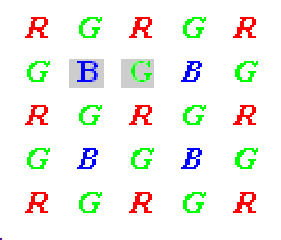
\includegraphics[width=1.89in,height=1.61in]{User1.pdf}}
\label{fig1}
\end{figure}

The output RGB components of a pixel are interpolated from 1, 2 or 4
neighbors of the pixel having the same color. There are several
modifications of the above pattern that can be achieved by shifting the
pattern one pixel left and/or one pixel up. The two letters C1 and C2 in the
conversion constants CV Bayer C1C2 2BGR and CV Bayer C1C2 2RGB indicate the
particular pattern type - these are components from the second row, second
and third columns, respectively. For example, the above pattern has very
popular ``BG'' type.

\newpage

\subsubsection{cv::ocl::integral}
\label{subsubsec:mylabel49}
Calculates the integral of an image.

Supports only CV{\_}8UC1 source type.

\textbf{image }The source image, $W\times H$, 8-bit or floating-point (32f or
64f)

\textbf{sum }The integral image, ($W$ + 1)$\times (H$ + 1), 32-bit integer or
floating-point (32f or 64f)

\textbf{sqsum }The integral image for squared pixel values, ($W$ + 1)$\times $
($H$ + 1), double precision floatingpoint (64f)

The functions integral calculate one or more integral images for the source
image as following:
\[
\mbox{sum}(X,Y)=\sum\limits_{x<X,y<Y} {\mbox{image}(x,y)}
\]
\[
\mbox{sqsum}(X,Y)=\sum\limits_{x<X,y<Y} {\mbox{image}(x,y)^2}
\]
\[
\mbox{tilted}(X,Y)=\sum\limits_{y<Y,abs(x-X+1)\le Y-y-1} {\mbox{image}(x,y)}
\]
Using these integral images, one may calculate sum, mean and standard
deviation over a specific up-right or rotated rectangular region of the
image in a constant time, for example:
\[
\sum\limits_{x_1 \le x<x_2 ,y_1 \le y<y_2 } {\mbox{image}(x,y)}
=\mbox{sum}(x_2 ,y_2 )-\mbox{sum}(x_1 ,y_2 )-\mbox{sum}(x_2 ,y_1
)+\mbox{sum}(x_1 ,y_1 )
\]
It makes possible to do a fast blurring or fast block correlation with
variable window size, for example. In the case of multi-channel images, sums
for each channel are accumulated independently.

As a practical example, the next figure shows the calculation of the
integral of a straight rectangle Rect(3,3,3,2) and of a tilted rectangle
Rect(5,1,2,3). The selected pixels in the original image are shown, as well
as the relative pixels in the integral images sum and tilted.

\begin{figure}[htbp]
\centerline{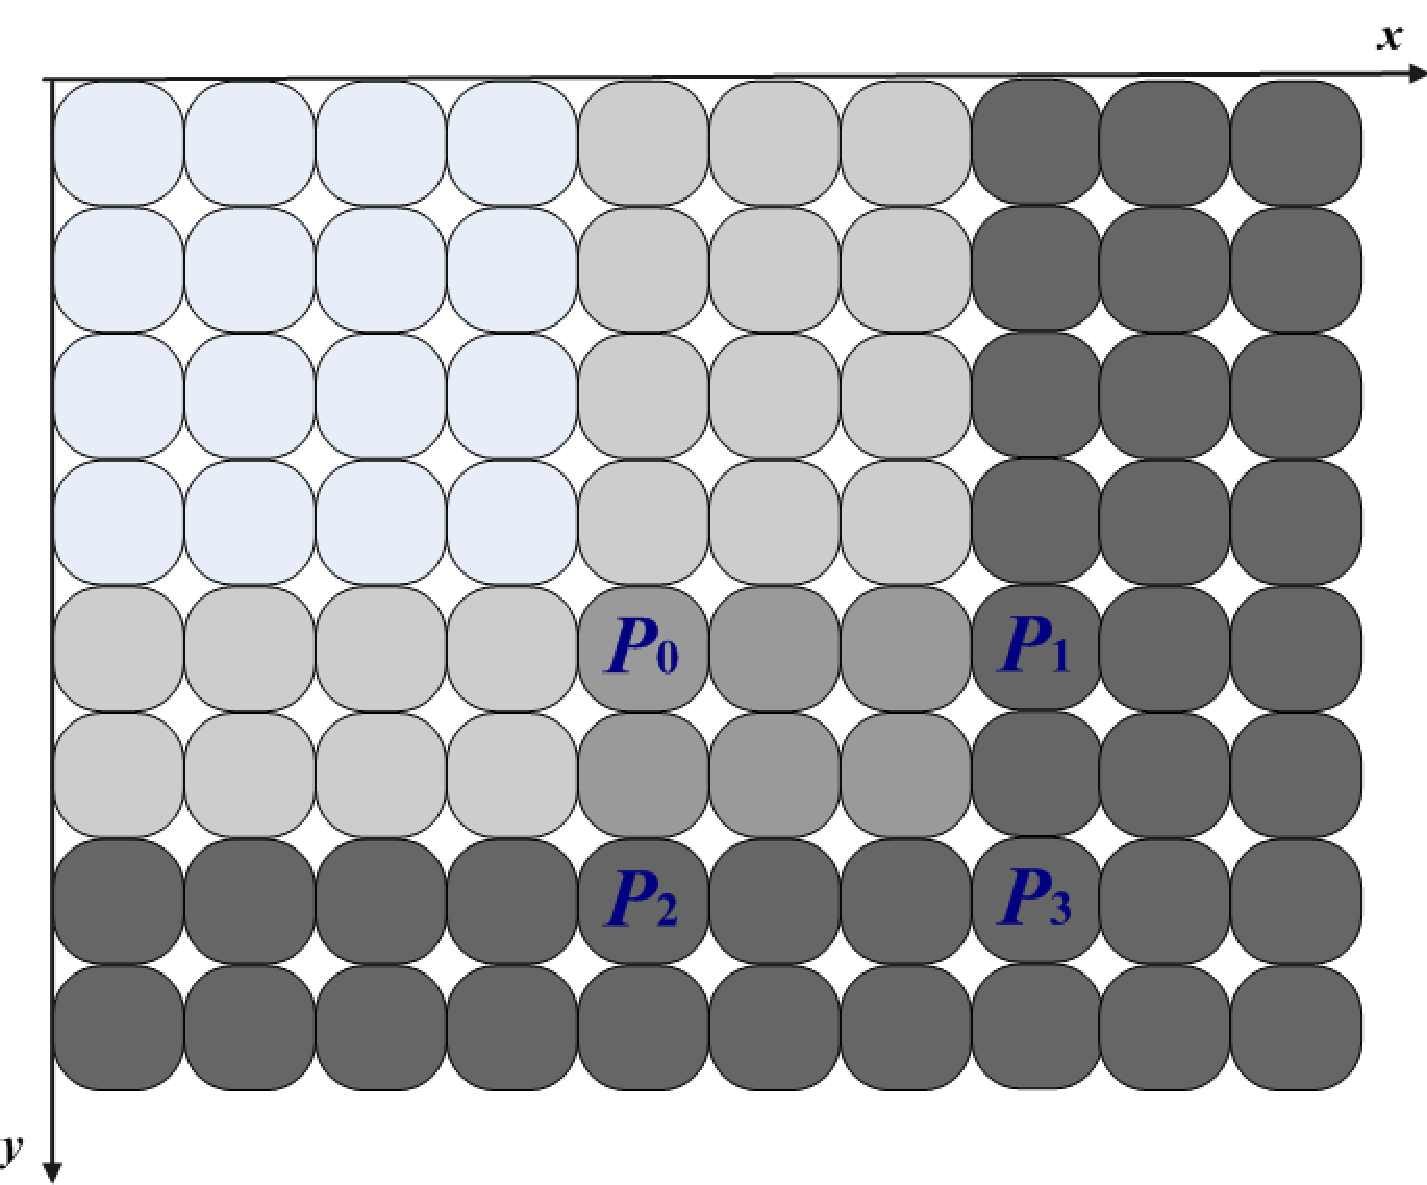
\includegraphics[width=7.15in,height=5.94in]{User2.pdf}}
\label{fig2}
\end{figure}

\begin{figure}[htbp]
\centerline{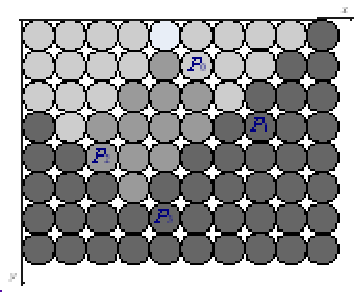
\includegraphics[width=2.38in,height=1.95in]{User3.pdf}}
\label{fig3}
\end{figure}
$\begin{array}{l}
 P_0 =\left\{ {y,x} \right\}=\left\{ {4,4} \right\} \\
 P_1 =\left\{ {y,x+w} \right\}=\left\{ {4,7} \right\} \\
 P_2 =\left\{ {y+h,x} \right\}=\left\{ {6,4} \right\} \\
 P_3 =\left\{ {y+h,x+w} \right\}=\left\{ {6,7} \right\} \\
 \end{array}$
\[
\begin{array}{l}
 P_0 =\left\{ {y,x} \right\}=\left\{ {1,5} \right\} \\
 P_1 =\left\{ {y+h,x+w} \right\}=\left\{ {3,7} \right\} \\
 P_2 =\left\{ {y+h,x-h} \right\}=\left\{ {4,2} \right\} \\
 P_3 =\left\{ {y+w+h,x+w-h} \right\}=\left\{ {6,4} \right\} \\
 \end{array}
\]
\newpage

\subsubsection{cv::ocl::threshold }
\label{subsubsec:mylabel50}
Applies a fixed-level threshold to each array element

Supports CV{\_}8UC1 and CV{\_}32FC1 data types.

\textbf{src }Source array (single-channel, 8-bit of 32-bit floating point)

\textbf{dst }Destination array; will have the same size and the same type as
src

\textbf{thresh }Threshold value

\textbf{maxVal }Maximum value to use with THRESH BINARY and THRESH BINARY
INV thresholding types

\textbf{thresholdType }Thresholding type (see the discussion)

The function applies fixed-level thresholding to a single-channel array. The
function is typically used to get a bi-level (binary) image out of a
grayscale image or for removing a noise, i.e. filtering out pixels with too
small or too large values. There are several types of thresholding that the
function supports that are determined by thresholdType:

\textbf{THRESH BINARY}
\[
\mbox{dst}(x,y)=\left\{ {{\begin{array}{*{20}c}
 {\max \mbox{Val}} & {\mbox{if src(x,y) > thresh}} \\
 0 & {\mbox{otherwise}} \\
\end{array} }} \right.
\]
\textbf{THRESH BINARY INV}
\[
\mbox{dst}(x,y)=\left\{ {{\begin{array}{*{20}c}
 0 & {\mbox{if src(x,y) > thresh}} \\
 {\max \mbox{Val}} & {\mbox{otherwise}} \\
\end{array} }} \right.
\]
\textbf{THRESH TRUNC}
\[
\mbox{dst}(x,y)=\left\{ {{\begin{array}{*{20}c}
 {\mbox{threshold}} & {\mbox{if src(x,y) > thresh}} \\
 {\mbox{src(x,y)}} & {\mbox{otherwise}} \\
\end{array} }} \right.
\]
\textbf{THRESH TOZERO}
\[
\mbox{dst}(x,y)=\left\{ {{\begin{array}{*{20}c}
 {\mbox{src(x,y)}} & {\mbox{if src(x,y) > thresh}} \\
 0 & {\mbox{otherwise}} \\
\end{array} }} \right.
\]
\textbf{THRESH TOZERO INV}
\[
\mbox{dst}(x,y)=\left\{ {{\begin{array}{*{20}c}
 \mbox{0} & {\mbox{if src(x,y) > thresh}} \\
 {\mbox{src(x,y)}} & {\mbox{otherwise}} \\
\end{array} }} \right.
\]
Also, the special value THRESH OTSU may be combined with one of the above
values. In this case the function determines the optimal threshold value
using Otsu's algorithm and uses it instead of the specified thresh. The
function returns the computed threshold value. Currently, Otsu's method is
implemented only for 8-bit images.

\begin{figure}[htbp]
\centerline{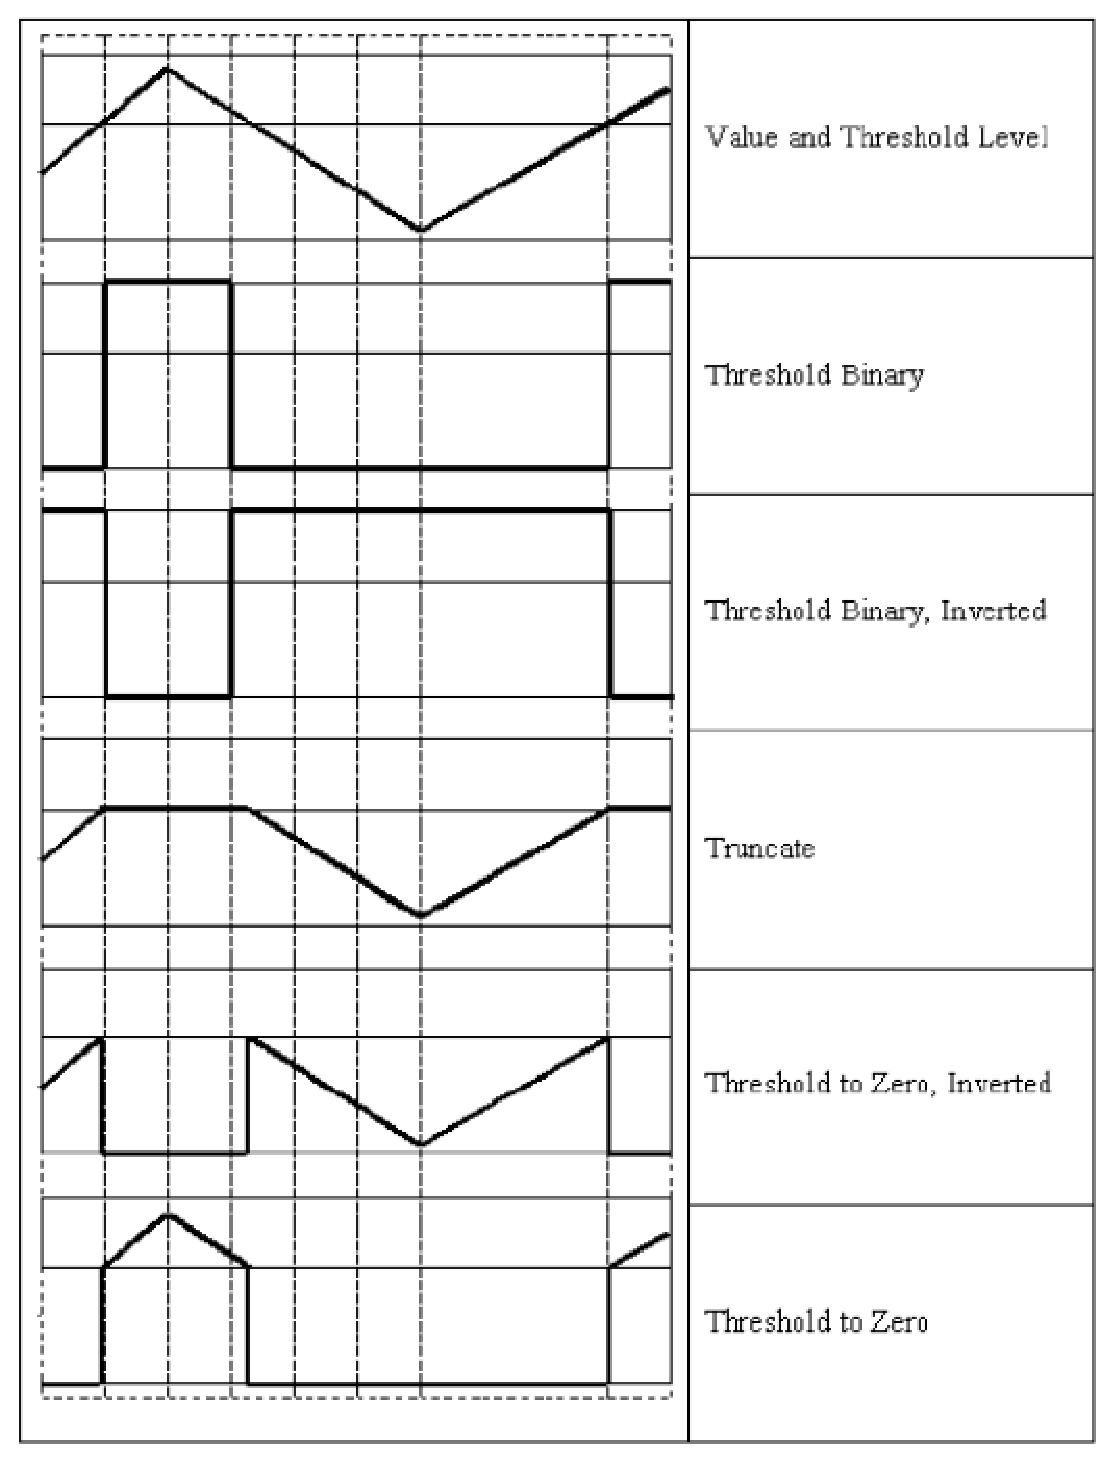
\includegraphics[width=5.55in,height=7.32in]{User4.pdf}}
\label{fig4}
\end{figure}

\end{document}
